% \documentclass[aspectratio=169,notes]{beamer}
\documentclass[aspectratio=169]{beamer}
\usetheme[faculty=phil]{fibeamer}
\usepackage{polyglossia}
\setmainlanguage{english} %% main locale instead of `english`, you
%% can typeset the presentation in either Czech or Slovak,
%% respectively.
\setotherlanguages{russian} %% The additional keys allow
%%
%%   \begin{otherlanguage}{czech}   ... \end{otherlanguage}
%%   \begin{otherlanguage}{slovak}  ... \end{otherlanguage}
%%
%% These macros specify information about the presentation
\title[AGLA2]{Analytical Geometry and Linear Algebra II, Lab 10} %% that will be typeset on the
\subtitle{Circulant Matrix \\ System of linear differential equations \\ \ 
         } %% title page.
\author{Oleg Bulichev}
%% These additional packages are used within the document:
\usepackage{ragged2e}  % `\justifying` text
\usepackage{booktabs}  % Tables
\usepackage{tabularx}
\usepackage{tikz}      % Diagrams
\usetikzlibrary{calc, shapes, backgrounds}
\usepackage{amsmath, amssymb}
\usepackage{url}       % `\url`s
\usepackage{listings}  % Code listings
% \usepackage{subfigure}
\usepackage{floatrow}
\usepackage{subcaption}
\usepackage{mathtools}
\usepackage{todonotes}
\usepackage{fontspec}
\usepackage{multicol}
\usepackage{pdfpages}
\usepackage{wrapfig}
\usepackage{animate}
\usepackage{booktabs}
\usepackage{multirow}

\graphicspath{{resources/}}
\frenchspacing

\setbeamertemplate{caption}[numbered]
\usetikzlibrary{graphs}

% \usepackage[backend=biber,style=ieee,autocite=footnote]{biblatex}
% \addbibresource{biblio.bib}
% \DefineBibliographyStrings{english}{%
%   bibliography = {References},}

\newcommand{\oleg}[2][] {\todo[color=red, #1] {OLEG:\\ #2}}
\newcommand{\fbckg}[1]{\usebackgroundtemplate{\includegraphics[width=\paperwidth]{#1}}}%frame background

\usepackage[framemethod=TikZ]{mdframed}
\newcommand{\dbox}[1]{
\begin{mdframed}[roundcorner=3pt, backgroundcolor=yellow, linewidth=0]
\vspace{1mm}
{#1}
\vspace{1mm}
\end{mdframed}
}

\begin{document}
\setlength{\abovedisplayskip}{0pt}
\setlength{\belowdisplayskip}{0pt}
\setlength{\abovedisplayshortskip}{0pt}
\setlength{\belowdisplayshortskip}{0pt}

\fbckg{fibeamer/figs/title_page.png}
\frame[c]{\setcounter{framenumber}{0}
    \usebeamerfont{title}%
    \usebeamercolor[fg]{title}%
    \begin{minipage}[b][6.5\baselineskip][b]{\textwidth}%
        \textcolor{black}{\raggedright\inserttitle}
    \end{minipage}
    % \vskip-1.5\baselineskip

    \usebeamerfont{subtitle}%
    \usebeamercolor[fg]{framesubtitle}%
    \begin{minipage}[b][3\baselineskip][b]{\textwidth}
        \raggedright%
        \insertsubtitle%
    \end{minipage}
    \vskip.25\baselineskip
}
%   \frame[c]{\maketitle}

\fbckg{fibeamer/figs/common.png}

\begin{frame}[c]{How I spent last weekend}
    \framesubtitle{}
    \vspace{-0.3cm}
    \begin{figure}[H]
        \begin{subfigure}{0.49\textwidth}
            \centering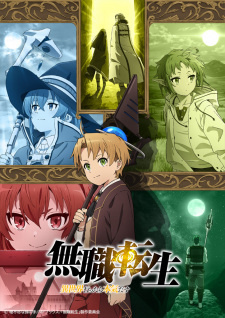
\includegraphics[height=5cm,width=1\textwidth,keepaspectratio]{mushoku_tensei.jpg}
            \caption*{\Large Watched both seasons in 1 day \\ (24 series) of "Mushoku Tensei"}
        \end{subfigure}
        \hfill
        \begin{subfigure}{0.49\textwidth}
            \centering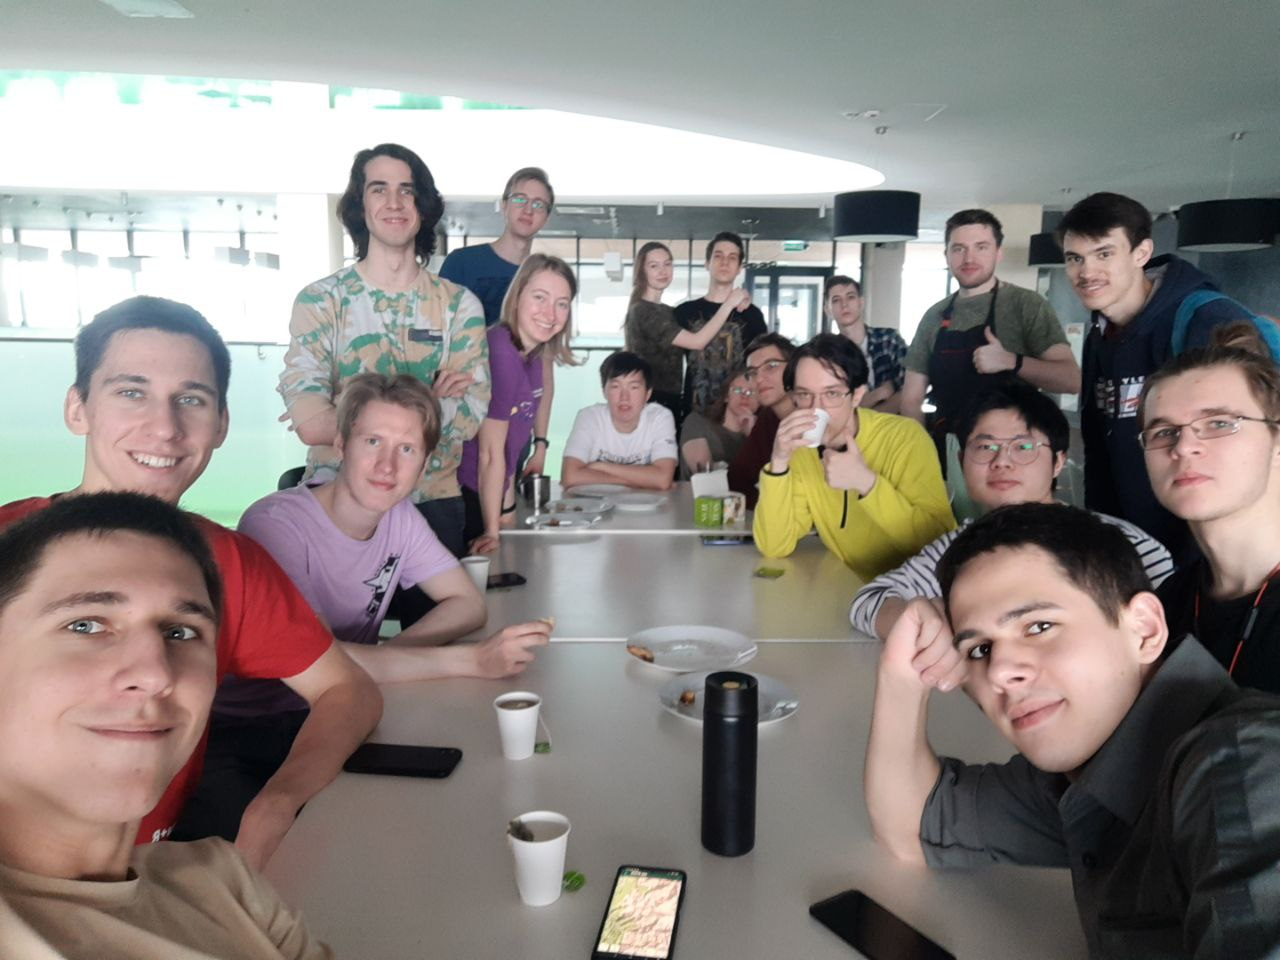
\includegraphics[height=5cm,width=1\textwidth,keepaspectratio]{rage_vegs.jpg}
            \caption*{\Large RAGE and VEGs clubs cooking collaboration event}
        \end{subfigure}
        
    \end{figure}
\end{frame}

\begin{frame}[t]{Circulant Matrix}
\framesubtitle{}
\textit{Watch first video on page \ref{itm:circulant}, if you want to look at derivation and the necessity of the matrix. }

\textbf{Circulant matrix ($N=4$) is:}
\begin{equation*}
    C_4 = c_0I+ c_1P + c_2P^2 + C_3P^3 = \begin{bmatrix}
    c_0 & c_1 & c_2 & c_3\\
    c_3 & c_0 & c_1 & c_2 \\ 
    c_2 & c_3  & c_0 & c_1 \\
    c_1 & c_2  & c_3 & c_0 
    \end{bmatrix}, \text{ where } P = \begin{bmatrix}
    0 & 1 & 0 & 0\\
    0 & 0 & 1 & 0 \\ 
    0 & 0  & 0 & 1 \\
    1 & 0  & 0 & 0 
    \end{bmatrix}
\end{equation*}
\textbf{Properties:} \\ 
It has \textbf{\textit{eigenvectors}} in the Fourier Matrix columns $F_4 = \begin{bmatrix}
1 & 1 & 1 & 1\\
1 & i & -1 & -i \\ 
1 & i^2  & 1 & (-i)^2 \\
1 & i^3  & -1 & (-i)^3 
\end{bmatrix}$ \\

\textit{\textbf{Eigenvalues}} of $C$ can be found by Fourier trans. $F_4[c_0,\ c_1,\ c_2,\ c_3]^T = [\lambda_0,\ \lambda_1,\ \lambda_2,\ \lambda_3]^T$
\end{frame}

\begin{frame}[t]{Circulant Matrix}
\framesubtitle{Example}
    \begin{figure}[H]
        \centering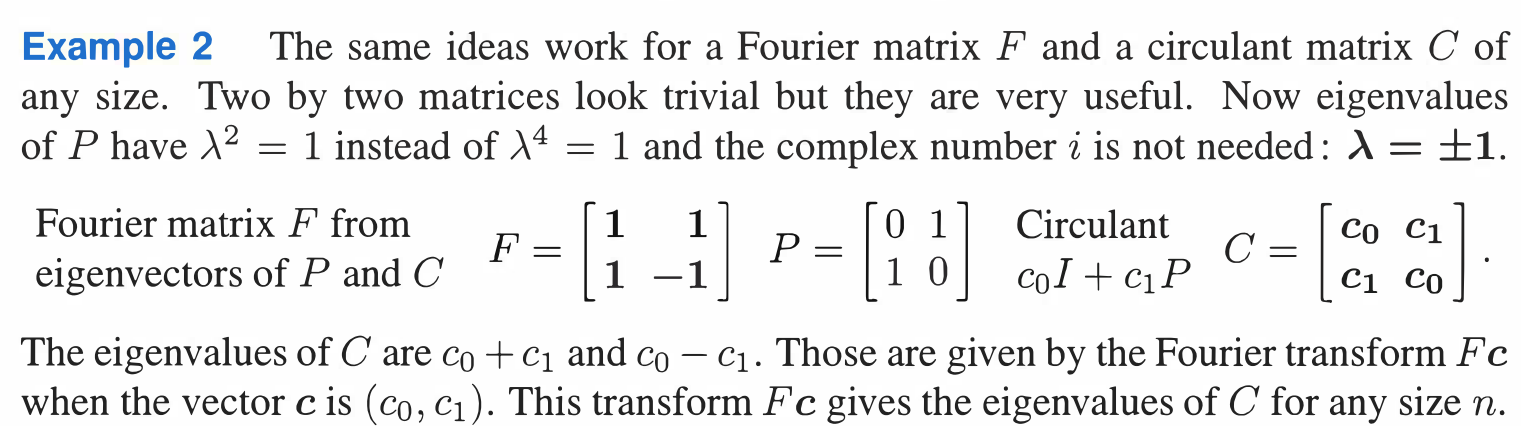
\includegraphics[height=6cm,width=1\textwidth,keepaspectratio]{circ_22.png}
        % \caption{caption_name}
        \label{fig:circ_22.png}
    \end{figure}
\end{frame}

\note{Эта тема на тестах у них была все время. Поэтому она тут.

Сделать упор, на то, что если они хотят понять смысл -- посмотреть видео Стренга.

Я на доске расписывал прям что на доске написано. Объяснял как записывать матрицу самому (каждая новая строка имеет последний элемент предыдущей и потом остальные в том же порядке что и наверху.)

Потом решали руками 2 на 2 и проверяли через классику(решение через собственные числа, а потом что получится при применении свойства.)

Разбирали, что если не понял тему фурье, то надо в читшит записать себе $F_{1-4}$, так как выше не будет 90 процентов}

\begin{frame}[t]{Task 1}
    \framesubtitle{}
    \vspace{-0.3cm}
    \only<1>{
    \begin{figure}[H]
        \centering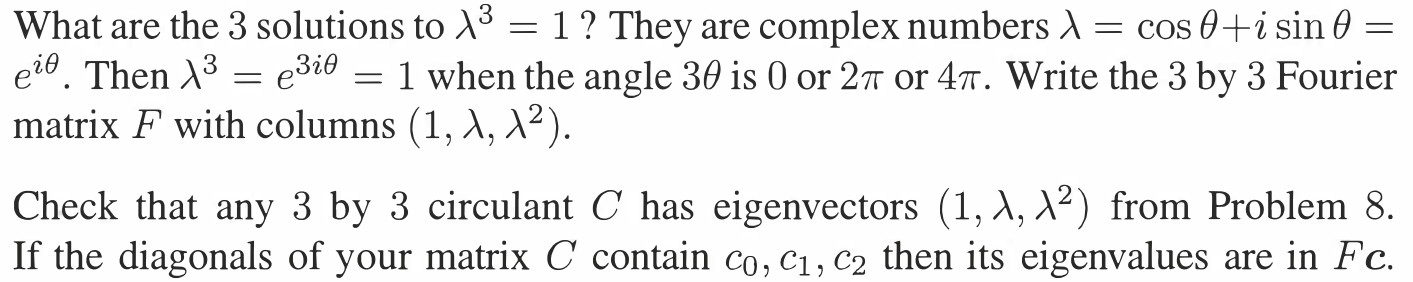
\includegraphics[height=5cm,width=1\textwidth,keepaspectratio]{1.png}
        % \caption{caption_name}
        \label{fig:1.png}
    \end{figure}
    }
    \only<2>{
        \alert{\Large Answer}
        \vspace{-1cm}
        \begin{figure}[H]
            \centering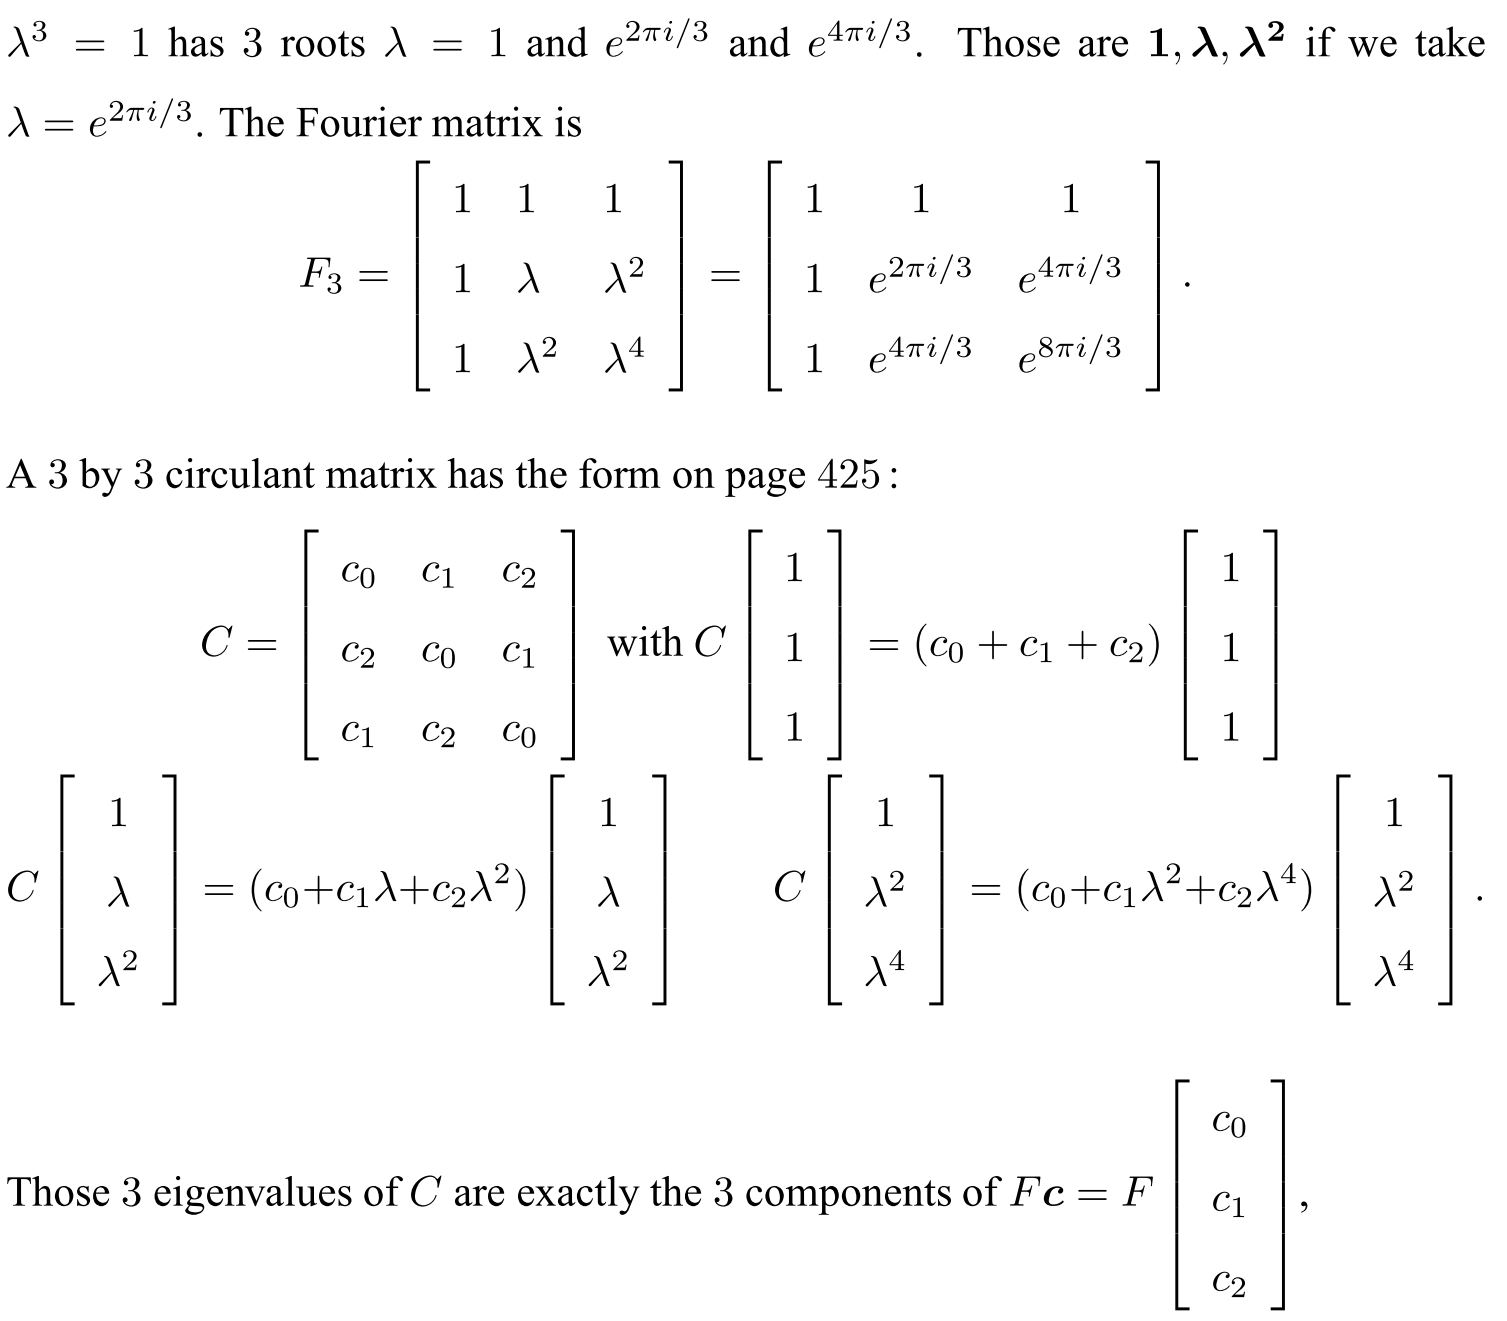
\includegraphics[height=7cm,width=1\textwidth,keepaspectratio]{1ans.png}
            % \caption{caption_name}
            \label{fig:1ans.png}
        \end{figure}
    }
\end{frame}

\note{Задачка простая, по факту делаем теперь 3 на 3. Но написано сложно. Поэтому и была добавлена, чтобы научились читать страшые текста.}

\begin{frame}[t]{1st order system of linear differential equations}
\framesubtitle{Algorithm}
\Large
\begin{enumerate}
    \item Write equation in $u' = Au$ form;
    \item Find eigenpairs of $A$
    \item Substitute  $\lambda$ and $x_{\lambda_i}$ to $u(t)=c_1e^{\lambda_1 t}x_1 + ... + c_ne^{\lambda_n t}x_n$
    \item Find all $c_i$ using $u(0)$ -- which is vector. $u(0) = \underbrace{u(t=0)}_{\text{from above}}$. Solve it.
    \item Put $c_i$ to $u(t)$.  
\end{enumerate}
\end{frame}

\note{Алгоритм объясняется на примере системы уравнений с лекции Стренга.

Делаю упор, что курс у вас будет потом, но сейчас важно понять только алгоритм. Стренг дал эту тему для того, чтобы вы поняли применение айгенов и все.}

\usebackgroundtemplate{}
\setbeamercolor{background canvas}{bg=}
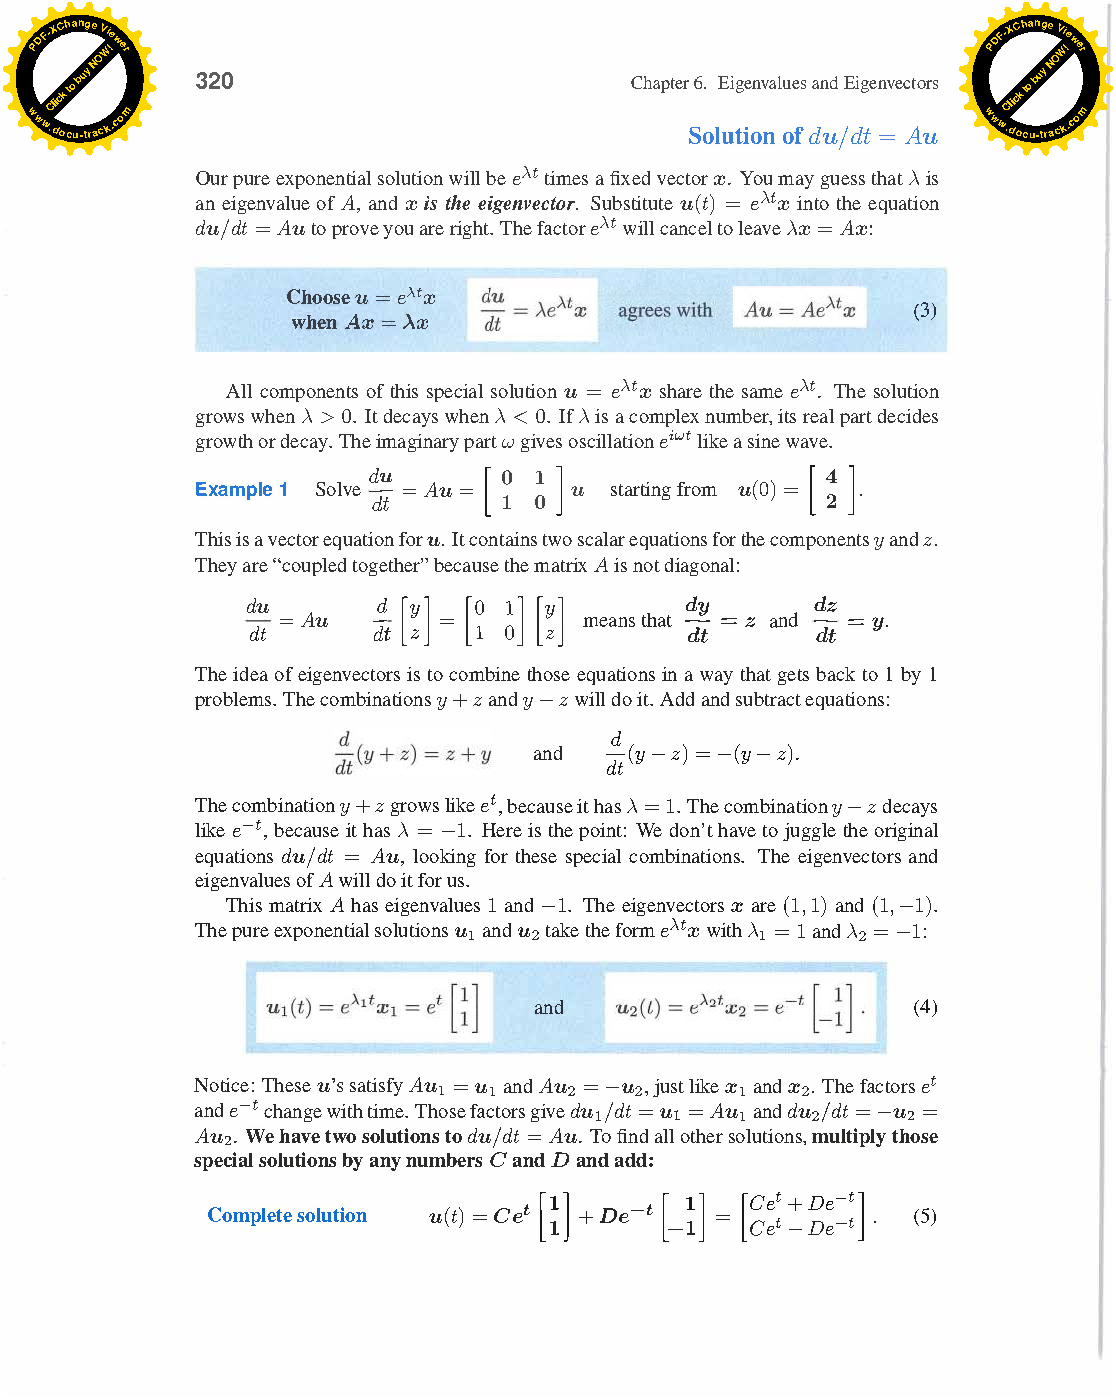
\includepdf[pages=-,fitpaper]{strang_book_1st_order.pdf}
\fbckg{fibeamer/figs/common.png}

\begin{frame}[t]{Task 2}
    \framesubtitle{}
    \vspace{-0.5cm}
    \begin{figure}[H]
        \centering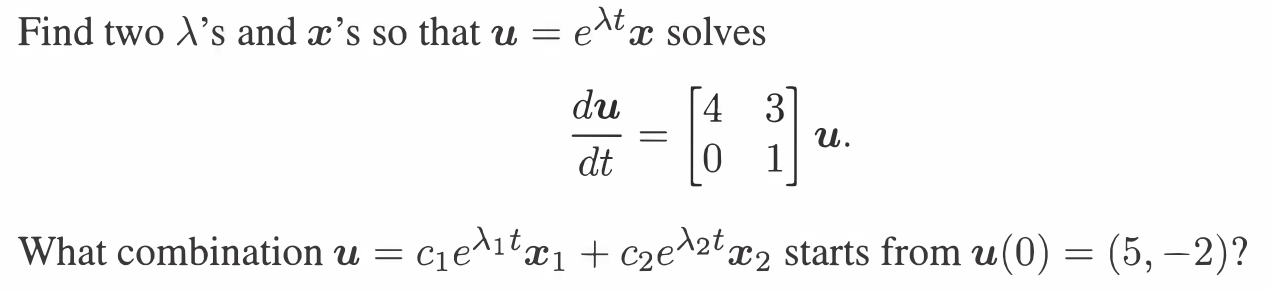
\includegraphics[height=3cm,width=1\textwidth,keepaspectratio]{2.png}
        % \caption{caption_name}
        \label{fig:2.png}
    \end{figure}
    \uncover<2->{
        \alert{\Large Answer}
        \vspace{-0.7cm}
        \begin{figure}[H]
            \centering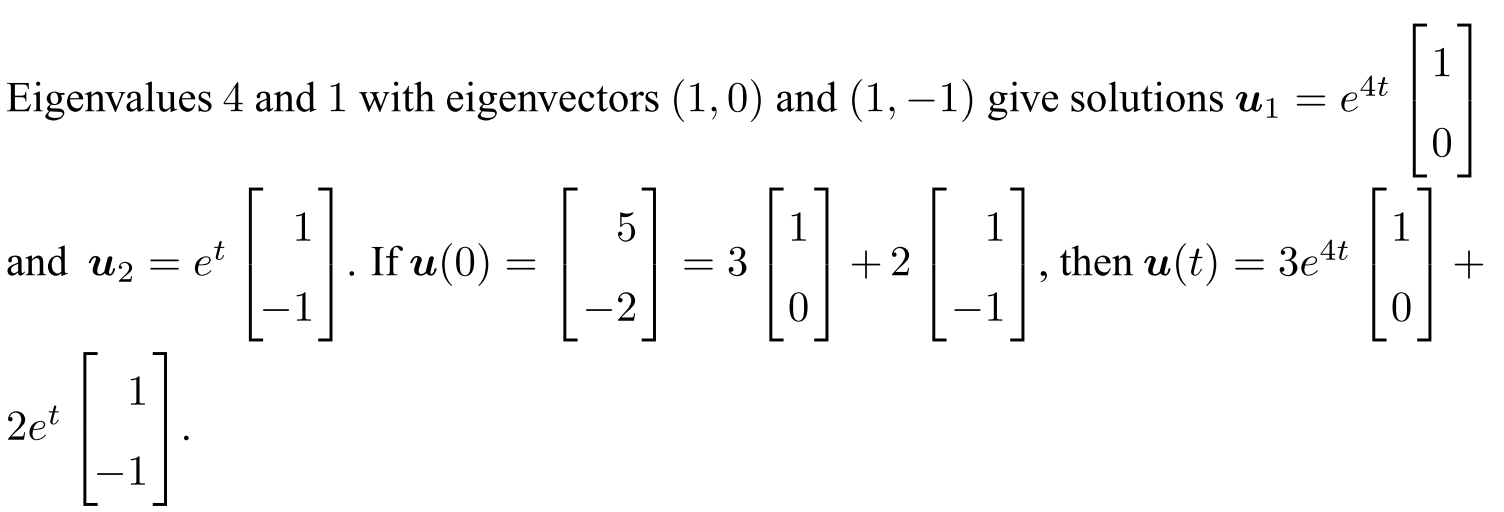
\includegraphics[height=3cm,width=1\textwidth,keepaspectratio]{2ans.png}
            % \caption{caption_name}
            \label{fig:2ans.png}
        \end{figure}
    }
\end{frame}

\begin{frame}[t]{Task 3}
    \framesubtitle{}
    \vspace{-0.5cm}
    \begin{figure}[H]
        \centering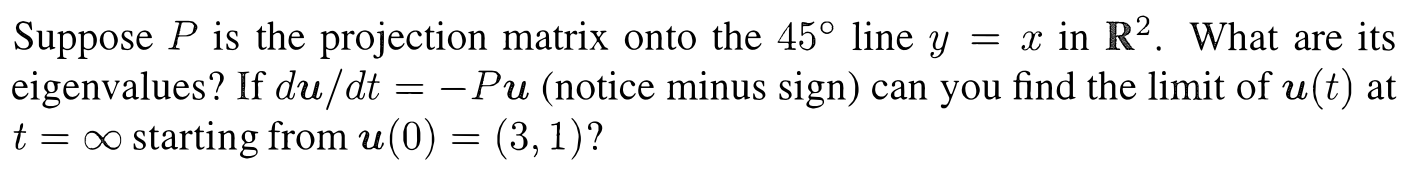
\includegraphics[height=3cm,width=1\textwidth,keepaspectratio]{3.png}
        % \caption{caption_name}
        \label{fig:3.png}
    \end{figure}
    \uncover<2->{
        \vspace{-1cm}
        \alert{\Large Answer}
        \begin{figure}[H]
            \centering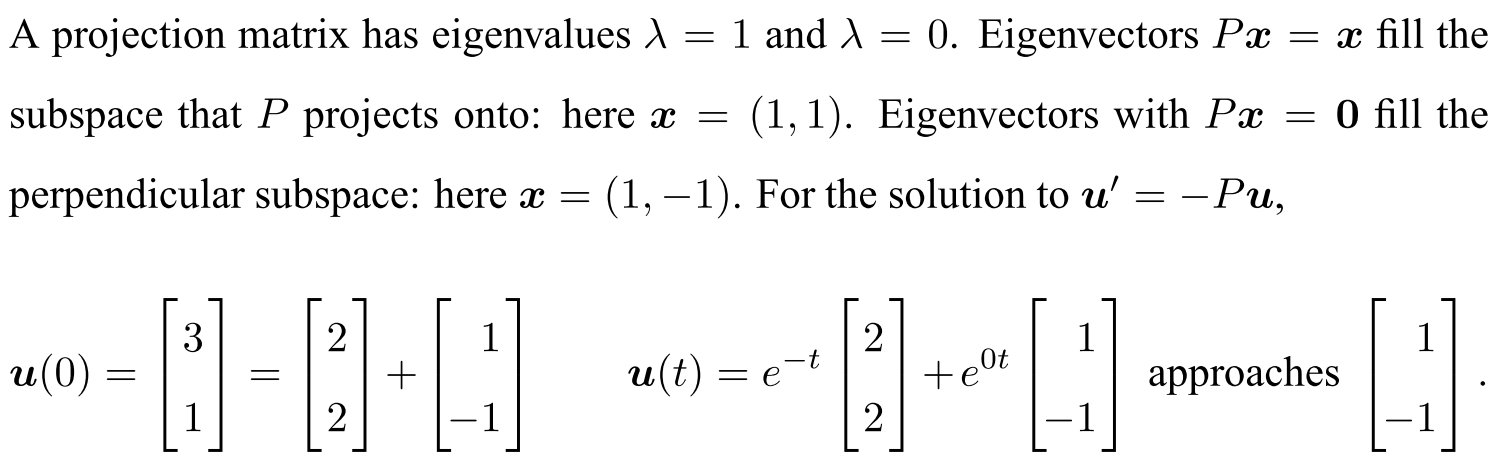
\includegraphics[height=4cm,width=1\textwidth,keepaspectratio]{3ans.png}
            % \caption{caption_name}
            \label{fig:3ans.png}
        \end{figure}
    }
\end{frame}

\note{Хорошая задача, чтобы вспомнить матрицу проекций. А так же расписать вместе с ними на доске, как надо читать задачу (какие таски надо сделать, не потерять минус итп.)

Последнее -- на пределе сделать уточнение.}

\begin{frame}[t]{Higher order differential equation}
\framesubtitle{Idea}
\Large
$$ u'' + Bu' + Cu = 0 \text{ is equivalent to } \begin{bmatrix}
u\\
u'
\end{bmatrix}' = \begin{bmatrix}
0 & 1\\ 
-C & -B 
\end{bmatrix} \begin{bmatrix}
u\\
u'
\end{bmatrix}$$
\\
Everything else is the same as in first order system.
\end{frame}

\note{Сделать упор на создание этой матрицы и про получение тривиального уравнения. Я сделал параллель с прошлой темой и поиском Фиббоначи. Студентам зашло.}

\usebackgroundtemplate{}
\setbeamercolor{background canvas}{bg=}
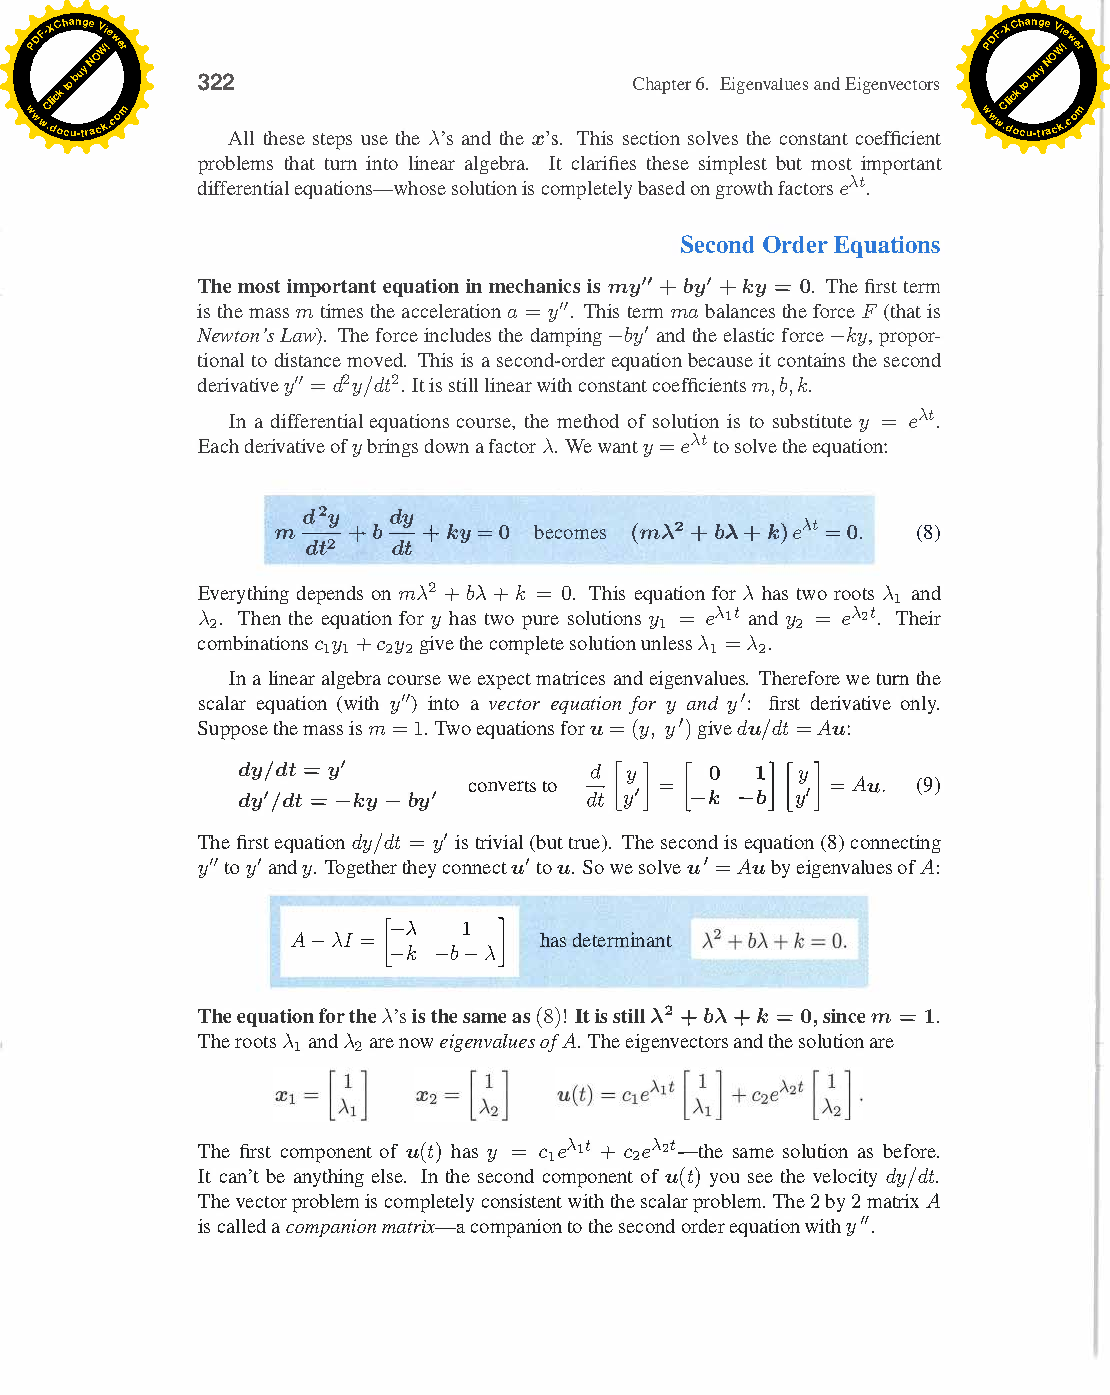
\includepdf[pages=-,fitpaper]{strang_book_2nd_order.pdf}
\fbckg{fibeamer/figs/common.png}

\begin{frame}[t]{Task 4}
    \framesubtitle{}
    \vspace{-0.5cm}
    \begin{figure}[H]
        \centering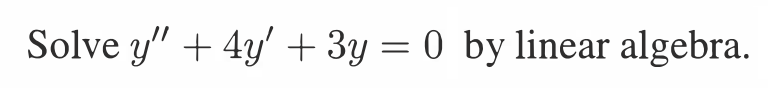
\includegraphics[height=1cm,width=1\textwidth,keepaspectratio]{4.png}
        % \caption{caption_name}
        \label{fig:4.png}
    \end{figure}
    \uncover<2->{
        \vspace{-0.5cm}
        \alert{\Large Answer}
        \vspace{-0.4cm}
        \begin{figure}[H]
            \centering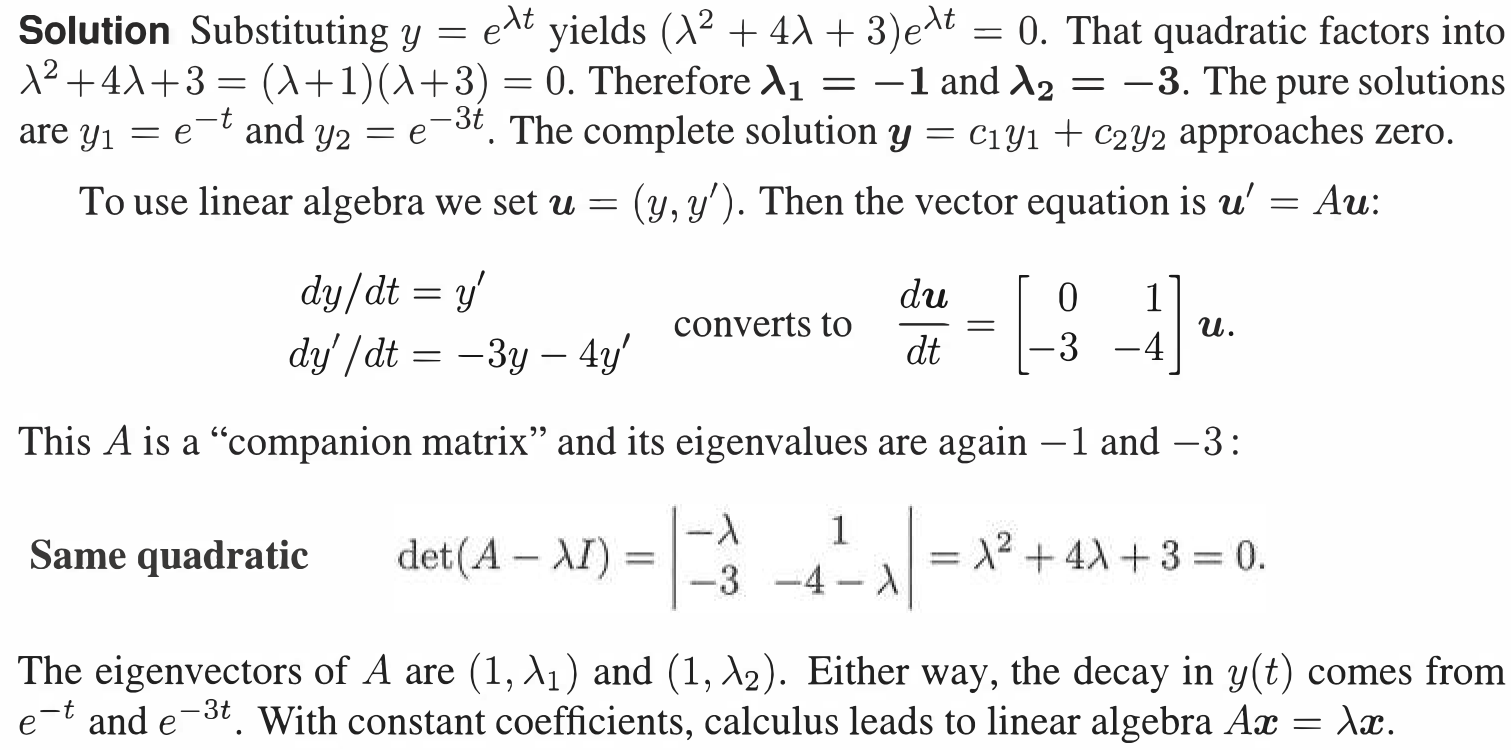
\includegraphics[height=5cm,width=1\textwidth,keepaspectratio]{4ans.png}
            % \caption{caption_name}
            \label{fig:4ans.png}
        \end{figure}
    }
\end{frame}

\begin{frame}[t]{Task 5}
    \framesubtitle{}
    \vspace{-0.3cm}
    \large
    \only<1>{
    Find solution in general form ($c_1e^{\lambda_1 t}x_1 + ... + c_ne^{\lambda_n t}x_n$):}
    \only<2>{\vspace{-0.8cm}}
    $$ u''' + 2u'' - u' - 2u = 0,\ u(0) = \begin{bmatrix}
    3\\
    2\\ 
    6
    \end{bmatrix}$$
    \only<2->{
        \alert{\Large Answer}
        \vspace{-0.5cm}
        \begin{enumerate}
            \item Equation: $\begin{bmatrix}
            y\\
            y'\\ 
            y''
            \end{bmatrix}' = \begin{bmatrix}
            0 & 1 & 0 \\
            0 & 0 & 1 \\ 
            2 & 1  & -2 
            \end{bmatrix}\begin{bmatrix}
                y\\
                y'\\ 
                y''
                \end{bmatrix}$;
            \item \vspace{-0.5cm} Eigenpairs: $\lambda_1 =-2,\ \lambda_2 =-1,\ \lambda_3 =1$; $x_1 = \begin{bmatrix} 1\\ -2\\ 4\end{bmatrix},\ x_2 = \begin{bmatrix} 1\\ -1\\ 1\end{bmatrix},\ x_3 = \begin{bmatrix} 1\\ 1\\ 1\end{bmatrix}$;
            \item \vspace{-0.5cm} $c_1 = 1,\ c_2 = -1,\ c_3= 3$;
            \item General form: $u(t) = 1e^{-2 t}\begin{bmatrix} 1\\ -2\\ 4\end{bmatrix} + (-1)e^{-1 t}\begin{bmatrix} 1\\ -1\\ 1\end{bmatrix} + 3e^{1 t}\begin{bmatrix} 1\\ 1\\ 1\end{bmatrix}$.
        \end{enumerate}
    }
\end{frame}

\note{Ее стоит порешать или хотя бы составить матрицу, так как не совсем тривиально это работает.}

\begin{frame}[t]{Reference material}
    \framesubtitle{}
    \Large
    \begin{itemize}
        \item \href{https://youtu.be/1pFv7e9xtHo}{Eigenvectors of Circulant Matrices: Fourier Matrix} \label{itm:circulant}
        \item \href{https://www.youtube.com/watch?v=IZqwi0wJovM&list=PL49CF3715CB9EF31D&index=23}{Lecture 23, Differential Equations and exp(At)}
        \item \textit{"Introduction to Linear Algebra", pdf pages 436 }\\ Circulant Matrix 8.3
        \item \textit{"Introduction to Linear Algebra", pdf pages 330--348 }\\ Systems of Differential Equations 6.3
    \end{itemize}
\end{frame}

\fbckg{fibeamer/figs/last_page.png}
\frame[plain]{}

\end{document}